\chapter{Implementation}

\section{Gas Costs Comparison}

In order to compare the gas consumption between implementations during testing we use eth-gas-reporter\footnote{\url{https://github.com/cgewecke/eth-gas-reporter}} which allows for to get gas usage per unit test, as well as retrieve average gas usage per method called. We configure \texttt{eth-gas-reporter} in the \texttt{truffle-config.js} file, and by prefixing a \texttt{truffle test} command with \texttt{GAS\_REPORTER=1} we can get enhanced tests as shown in Figure \ref{fig:gas-reporter}. The metrics shown in Table \ref{table:compare-gas} are obtained after running the 4 tests in the supplied \texttt{smartcontract-gascomparison} repository.

\begin{figure}[htb]
    \centering
    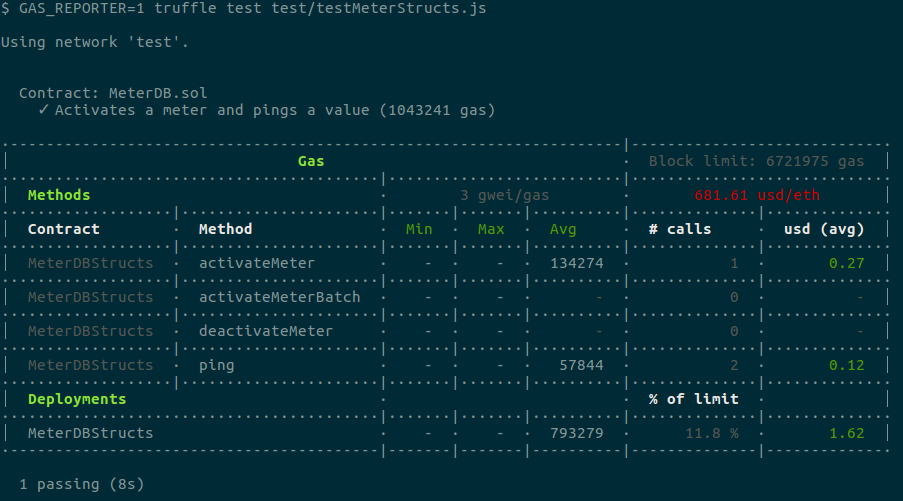
\includegraphics[width=\textwidth]{gas-reporter}
    \caption{Running a truffle test with eth-gas-reporter}
    \label{fig:gas-reporter}
\end{figure}

\section{Access Control}\label{apx:implementation:acl}
Explain modifiers and whitelist. Compare to having ACL contract.

In this section we further explain how the logic of the Access Control List from DAppHub works. Cite  https://github.com/dapphub/ds-roles

\section{Listening for Events} \label{apx:implementation:events}

In order to fetch all the past readings of a meter we implement some js scripts to allow fetching all past events. <describe implementation>
These techniques can be used for rendering the info on a react webpage.
